\chapter{Anwendung}

\begin{figure}[h!]
    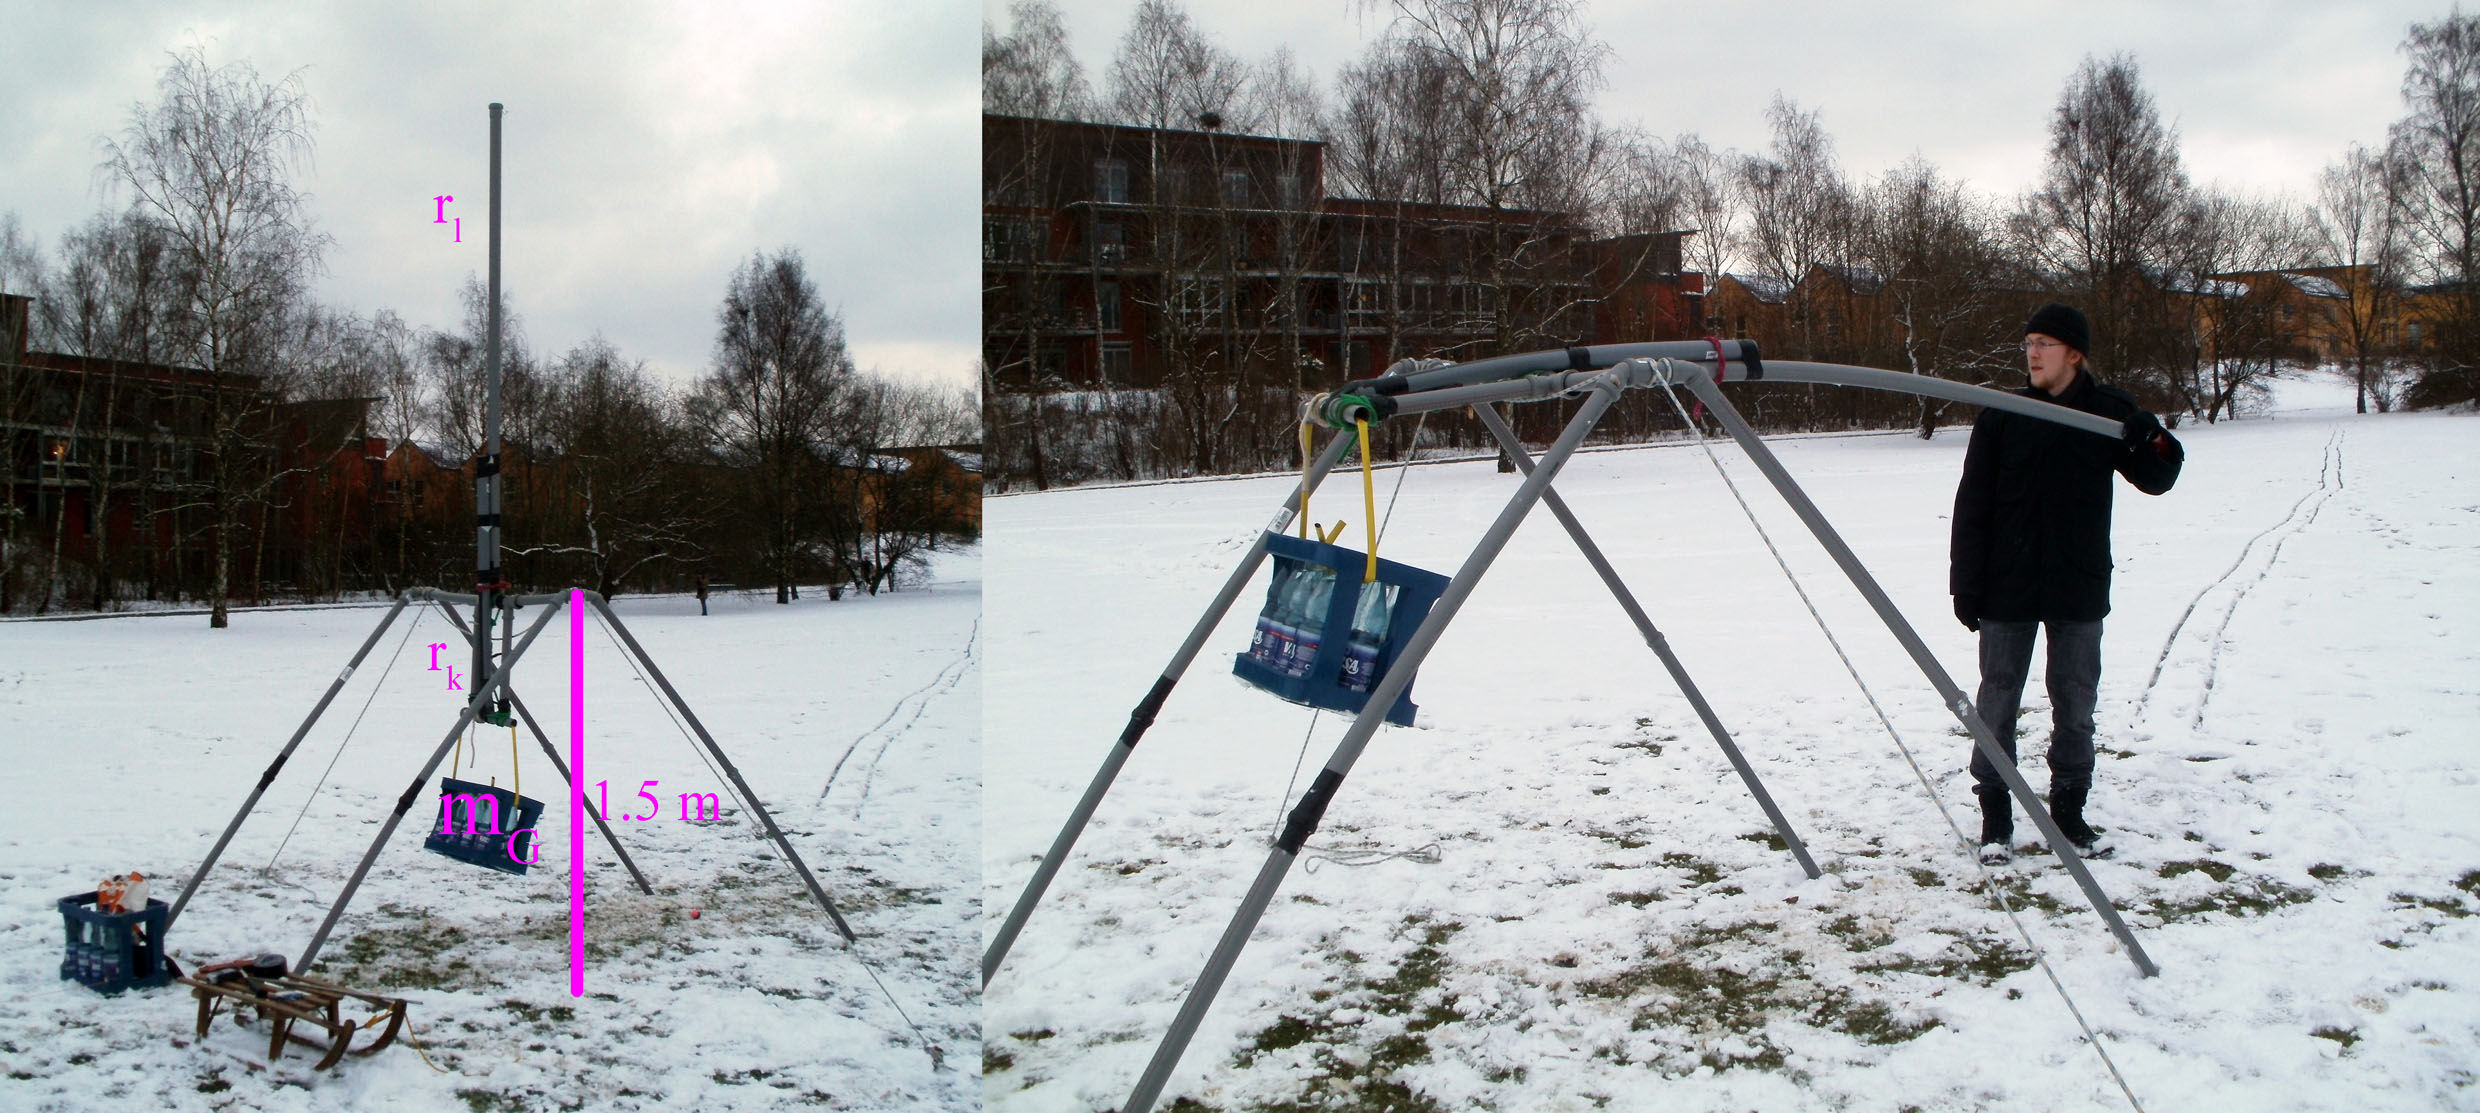
\includegraphics[width=\textwidth]{bilder/trebuchet-final}
    \caption{Links: Die Konstruktion des Trebuchets. Rechts: Der Autor spannt das Trebuchet.}
\end{figure}


\section{Variablendeklaration}
Um Unklarheiten in der Benennung von Variablen im Vorhinein zu vermeiden, ist es am besten, sämtliche Variablennamen ganz auszuschreiben (z.B. $m_{Geschoss}$). Dadurch werden jedoch viele Terme, insbesondere in (\ref{starre-koerper}), unleserlich. Deswegen habe ich mich für einen, maximal zwei Buchstaben pro Objekt entschlossen. Folgende, nicht selbsterklärende Indices werden verwendet:
\begin{description}
\item[$_k$] Der kurze Hebelarm, an dem das Gegengewicht befestigt ist.
\item[$_l$] Der lange Hebelarm, an dessen Ende sich das Geschoss befindet.
\item[$_{lk}$] Der gesamte Hebelarm.
%\item[$_{LK}$]Der gesamte Arm des Hebels.
\item[$_P$] Das Geschoss (abgeleitet von Projektil).
\item[$_G$] Das Gegengewicht.
\end{description}
Wenn eine Variable auch ohne Index einen eindeutigen Namen besitzt (etwa das Drehmoment $M$), wird der Index ausgelassen.

\label{energie-allgemein}
\section{Erste Abschätzungen mithilfe der allgemeinen Energieerhaltung}

Bei vielen Problemen in der Mechanik ist es ausreichend oder zumindest hilfreich zu versuchen, das Problem mithilfe der Energieerhaltung zu formulieren, um eine erste Abschätzung vornehmen zu können. 

\paragraph{Energie des Wurfarmes.}
So auch hier: Zunächst bestimmen wir die Gesamtenergie, die wir dem Trebuchet zuführen:
\begin{align}
\label{gesammtenergie}
E_{ges} &= m_G g h_0 %\emph{Anfängliche, potentielle Energie des Trebuchets}
\end{align}
Dabei ist $h_0$ die Höhe und $m_G$ die Masse des Gegengewichtes. Wenn wir davon ausgehen, dass das Geschoss in dem Moment freigegeben wird, in dem das Gegengewicht seine tiefste Stelle erreicht (also wenn $h=0$ gilt), wird diese Energie auch bestmöglich genutzt.
Man könnte jetzt (vorschnell) schlussfolgern, dass die Reichweite des Trebuchets direkt von $E_{ges}$ abhinge, also $E_{ges}=E_P$ sei. Jedoch schwingt der Wurfarm nach Abwurf des Geschosses weiter. Dafür ist natürlich auch Energie notwendig, die dann nicht mehr dem Geschoss zur Verfügung stehen kann.
Natürlich gibt es auch keine lineare Abhängigkeit, also etwa $E_P=\frac{m_P}{{m_{Trebuchet}}} E_{ges}$, denn der Wurfarm hat an verschiedenen Stellen eine unterschiedliche Geschwindigkeit und deswegen auch eine unterschiedlich hohe, kinetische Energie.

\paragraph{Energie des Geschosses.}
Die Reichweite $s$ des Trebuchets hängt hauptsächlich von der Anfangsgeschwindigkeit und so von der anfänglichen, kinetischen Energie des Geschosses ab:
\begin{align}
\label{wurfweite}
s &= \frac{v_{0, P}^2 \sin{2\varphi_P}} {g} \\%\emph{Wurfweite des schiefen Wurfes (ohne Luftwiederstand)}\\
E_P &= \frac{m_P v_P^2}{2} %\emph{Kinetische Energie des Geschosses}
\end{align}
Wenn man die Luftreibung vernachlässigt und den Abwurfwinkel $\varphi_P=\frac{\pi}{4}$ setzt, um die maximale Reichweite zu erzielen (ein Winkel von $0$ entspricht der Waagerechten), ergibt sich durch Äquivalenzumformung sofort die Reichweite in Abhängigkeit von der Energie:
\begin{align}
s(E) &= \frac{2 E_P}{ m_P}\frac{\sin{2\varphi_P}}{g}%\emph{Reichweite des Trebuchets}
\end{align}
Damit ist klar, dass für die reale Reichweite $s_{real}$ in jedem Fall
\begin{align}
s_{real}&<s(E_{ges})
\end{align}
gelten muss. Mehr Informationen können mit der einfachen Energieerhaltung noch nicht gewonnen werden (die Verbesserung wird in (\ref{energie-rot}) vorgenommen).
\section{Berechnung als starrer Körper}
\label{starre-koerper}
Um die tatsächliche Abwurfgeschwindigkeit und damit die Reichweite des Trebuchets zu bestimmen, ist es nun notwendig, den Wurfarm als starren Körper anzusehen.

\paragraph{Das Drehmoment des Gegengewichtes.}
An einem Ende des Wurfarms (bzw. Hebelarms, denn physikalisch ist dieser nichts anderes) greift die Gewichtskraft des Gegengewichts an. Beim Schwingen zwingt der Wurfarm das Gegengewicht auf eine Kreisbahn. Es liegt also ein Drehmoment vor, welches vom Winkel des Wurfarmes abhängt, denn die Gewichtskraft des Gegengewichts zeigt immer nach unten, während der Wurfarm seinen Winkel verändert:
\begin{align}
F &= m_G g \cos{\varphi}\\
\label{drehmoment}
\vec M &=\vec r_k \times \vec F_G
\end{align}
Dabei beschreibt $\varphi=0$ die Waagerechte.

\paragraph{Das Trägheitsmoment des Wurfarms.}
Um die Beschleunigung des Wurfarms zu bestimmen, muss dessen Trägheitsmoment bekannt sein. Der Wurfarm wird dazu zu einem Quader von homogener Dichte $\varrho$ vereinfacht, der den Querschnitt $A =a b$ und die Länge $r=r_k+r_l$ besitzt\footnote{Natürlich gilt $m_{lk}=\varrho A r$}. Ein Blick in die Formelsammlung oder ein einfaches Volumenintegral\footnote{Für Berechnung siehe Anhang} liefert folgendes:
\begin{align}
\label{I_mod}
I_1= m_{lk} \frac{r^2+b^2}{12}
\end{align}
Dabei bleibt jedoch die Lage der Rotationsachse unberücksichtigt: Diese muss nicht mit der Symmetrieachse des Wurfarmes (wie $I_1$ suggeriert) zusammenfallen. Etwa bei historischen Trebuchets liegt sie bei $\frac{1}{6}r$. Um (\ref{I_mod}) entsprechend zu modifizieren, wird der \emph{Steiner'sche Verschiebungssatz} verwendet:
\begin{align}
\label{r_rot}
\Delta r_{rot}&=\frac{r}{2}-(r_l-r_k)\\
\label{traegheitsmoment-n2}
I_2 &= m_{lk} \frac{r^2+b^2}{12} + m_{lk} (\Delta r_{rot})^2
\end{align}
In (\ref{r_rot}) wird die Entfernung der Symmetrieachse zur tatsächlichen Rotationsachse berechnet. Bisher wurde nur das Trägheitsmoment des Arms berechnet, jedoch nicht das des Geschosses. Dieses kann hier gut durch das Trägheitsmoment einer Punktmasse am Ende des Wurfarmes repräsentiert werden, welches einfach zu $I_2$ addiert wird:
\begin{align}
\label{traegheitsmoment}
I&=m_{lk} \frac{r^2+b^2}{12} + m_{lk} (\Delta r_{rot})^2+m_P r_l^2
\end{align}
Warum beeinflusst das Gegengewicht des Trebuchets $I$ nicht? Das Gegengewicht gibt die Geschwindigkeit des Arms vor: Der Arm des Trebuchets kann natürlich niemals schneller werden als das fallende Gegengewicht. Oder anders ausgedrückt: Die Trägheit des Gegengewichts spielt keine Rolle, da es niemals durch den Arm beschleunigt wird, sondern nur durch die Gravitationskraft.

\label{endgesch-starr}
\paragraph{Die Endgeschwindigkeit.}
Mit den Formeln (\ref{drehmoment}) und (\ref{traegheitsmoment}) kann nun die allgemeine Bewegungsgleichung aufgestellt werden, es gilt (\ref{rotationsbeschleunigung}):
\begin{align}
M = r_k m_G g \cos{\varphi}  &= I \dot{\omega}\\
\Leftrightarrow g  \cos{(\varphi(t))} \frac{r_k m_G}{I} &=\diff{\omega(t)}{t}\\
\label{bewegungsgleichung_i}
\approx  \varsigma g\frac{r_k m_G}{I} &=\diff{\omega(t)}{t}
\end{align}
Hier wird ein grundlegendes Problem deutlich: Die Bewegungsgleichung enthält den Kosinus ihrer eigenen (zweifachen) Aufleitung. Die Lösung der sich daraus ergebenden Differentialgleichung würde sowohl den mathematischen Rahmen dieser Facharbeit sprengen als auch die Nachvollziehbarkeit der weiteren Rechnung erheblich beeinträchtigen.
Deswegen wird die \emph{Vereinfachung} $\cos{\varphi}\approx \varsigma$ mit $\varsigma=0.77$ für $0\le\varphi\le\frac{\pi}{2}$ vorgenommen
\footnote{Das ergibt sich aus dem Mittelwert des Kosinus, gewichtet in Richtung $\varphi=0$, denn der beschleunigende Wurfarm hält sich viel länger bei $0\le\varphi\le\frac{\pi}{4}$ als bei $\frac{\pi}{4}\le\varphi\le\frac{\pi}{2}$ auf:
 $\frac{ \frac{
 		\int_
 			{0} ^\frac{\pi}{2} 
 			\cos{\varphi}\mathrm d\varphi}{
 			\frac{\pi}{2}
 		} +
 		 \frac{
 		\int_
 			{0} ^\frac{\pi}{4} 
 			\cos{\varphi}\mathrm d\varphi
 		}{
 			\frac{\pi}{4}
 		}}{2}\approx 0.77 $
}.
Wenn man (\ref{bewegungsgleichung_i}) jetzt nach der Zeit integriert, erhält man die Winkelgeschwindigkeit, nochmaliges Integrieren führt zum Winkel des Wurfarmes:
\begin{align}
\nonumber
\int\diff{\omega(t)}{t}{\mathrm d t}=&\int{\varsigma g\frac{r_k m_G}{I}}{\mathrm d t}=\\
\label{gesch_zeit}
\omega(t)=&\varsigma g\frac{ r_k m_G}{I}t\\
\nonumber
\Leftrightarrow \int{\omega(t)}\mathrm d t=&\int{\varsigma g\frac{r_k m_G}{I}t}{\mathrm d t}=\\
\label{weg_zeit}
\varphi(t)=&\varsigma g\frac{r_k m_G}{2I}t^2
\end{align}
Dabei ist der Winkel des Wurfarmes relativ zur Horizontalen, d.h. $\varphi=0$ ist waagerecht. Um die Endwinkelgeschwindigkeit $\omega_{e}$ zu erhalten, muss man nun (\ref{weg_zeit}) nach $t$ umformen und in (\ref{gesch_zeit}) einsetzen\footnote{Für genaue Äquivalenzumformung siehe Anhang}. Dann kann man nach (\ref{umfangsgeschwinigkeit}) die Abwurfgeschwindigkeit des Geschosses errechnen, welches sich bei $r_l$ befindet:
\begin{align}
\omega(\varphi)=&\varsigma g\frac{ r_k m_G}{I}\sqrt{\frac{2\varphi}{\dot\omega}}\\
v_{0,P}=&\varsigma g\frac{ r_l r_k m_G}{I}\sqrt{\frac{2\varphi}{\dot\omega}}
\end{align}
Das so errechnete $v_{0,P}$ wird in (\ref{wurfweite}) eingesetzt und mit (\ref{bewegungsgleichung_i}) vereinfacht,
\begin{align}
\nonumber
s =& \frac{2 \varphi_{lk} \varsigma^2 g^2 m_G^2 r_l^2 r_k^2 \sin{(2\varphi_P)}}{\dot\omega I^2 g}\\\nonumber
  =& \frac{2 \varphi_{lk} \varsigma^2 g^2 m_G^2 r_l^2 r_k^2 \sin{(2\varphi_P)}}{\varsigma g\frac{r_l m_k}{I} I^2 g}\\
  =&  2\varphi_{lk}\varsigma\sin{(2\varphi_P)} \ \  \frac{m_G r_k r_l^2 }{I}
\end{align}
um dann mit (\ref{traegheitsmoment}) und weitere Vereinfachung auf die Reichweite des Trebuchets zu kommen:
\begin{align}
\nonumber
s =& 2\varphi_{lk} \varsigma \sin{(2\varphi_P)} \ \ \frac{ m_G  r_kr_l^2 }
		{m_{lk} \frac{r^2+b^2}{12} + m_{lk} (\frac{r}{2}-(r_l-r_k))^2+m_P r_l^2}\\
		\label{reichweite}
  =& 2 \varphi_{lk} \varsigma \sin{(2\varphi_P)} \ \ \frac{ m_G  r_kr_l^2}
		{m_{lk} \frac{r^2+b^2}{12} + m_{lk} (\frac{3r_k-r_l}{2})^2+m_P r_l^2}
\end{align}

\paragraph{Deutung.}
Dieser Term besteht aus verschiedenen, mit einander \glqq konkurrierenden\grqq \ Ausdrücken: Um eine maximale Reichweite zu erreichen, muss $\varphi_P$ möglichst $45^\circ$ sein ($\sin{(2\varphi_P)}=1$), während $\varphi_{lk}$ möglichst $90^\circ$ betragen sollte, da der Hebelarm bis zu diesem Punkt das Geschoss (in Schussrichtung) beschleunigen kann (danach wird es verzögert, denn das Gegengewicht wird wieder angehoben). Mit einem einfachen Hebelarm (bei dem $\varphi_P=\varphi_{lk}$) ist nur ein Kompromiss erreichbar, weswegen bei vielen echten Trebuchets das Geschoss über ein Seil mit dem Wurfarm verbunden ist. Da das Geschoss nicht sofort beschleunigt wird, sondern erst das Seil gestrafft werden muss, ist $\varphi_P<\varphi_{lk}$. Ein positiver Nebeneffekt ist, dass das Seil $r_l$ vergrößert, ohne jedoch das Trägheitsmoment nennenswert zu steigern, da $m_{Seil}<<m_l$. Das \glqq hinterherhinkende\grqq \ Seil zu berechnen ist indes doch recht komplex, weswegen es hier nicht berücksichtigt wird.

Zwei weitere konkurrierende Faktoren sind die Länge der Hebelarme und ihre Trägheitsmomente: Ein größeres $r_k$ erhöht natürlich das Drehmoment des Gegengewichtes und kann das Geschoss also besser beschleunigen. Deswegen steht $r_k$ im Zähler. Aber ein größeres $r_k$ führt natürlich auch zu einem größeren $m_k$, was das Trägheitsmoment erhöht. Das wiederum verringert die Beschleunigung des Geschosses. Deswegen steht $r_k$ auch im Nenner. Das gleiche gilt natürlich auch für $r_l$.

In der Praxis ist es also wichtig, $m_{lk}$ möglichst klein gegenüber $m_P$ zu halten, ohne jedoch auf einen großen Hebel ($r$) zu verzichten. Darin liegt auch die Schwierigkeit, ein gutes Trebuchet zu bauen: Wie man dem Term ansieht, ist es nicht ohne weiteres möglich, ein Maximum auszurechnen.
\section{Berechnung mithilfe der Energieerhaltung unter Berücksichtigung der Rotationsmechanik}
\label{energie-rot}
Der bisherige Rechenweg ist recht aufwändig gewesen. Vielleicht bietet die Energieerhaltung einen einfacheren Lösungsweg, wenn man sie um die Erhaltung der Rotationsenergie erweitert (\ref{rotationsenergie})?

\paragraph{Energie des Wurfarmes.}
Gleichung (\ref{gesammtenergie}) gilt natürlich weiterhin; die Energie des Wurfarmes wird diesmal aber auch durch die Rotationsenergie ausgedrückt:
\begin{align}
E_{ges}=\frac{I\omega^2}{2}
\end{align}
Damit wird es möglich, die Energie auszurechnen, die dem Trebuchet verloren geht, wenn das Geschoss sich löst. Dafür werden die unterschiedlichen Trägheitsmomente (\ref{traegheitsmoment-n2}, \ref{traegheitsmoment}) gebraucht, die schon im vorherigen Unterkapitel ausgerechnet worden sind:
\begin{align}
\Delta I &= I-I'= m_P r_l^2\\
\frac{I\omega^2}{2}&=\frac{I'\omega^2}{2}+E_P\\
\Leftrightarrow E_P&=\frac{\omega^2}{2}\Delta I 
\end{align}
Damit und mit den Erkenntnissen aus (\ref{energie-allgemein}) kann die Reichweite beschrieben werden:
\begin{align}
\nonumber
s(E_P)&= \frac{2 \frac{\omega^2}{2}\Delta I}{ m_P}\frac{\sin{2\varphi_P}}{g}\\
	  &= \frac{\omega^2 m_P r_l^2}{ m_P}\frac{\sin{2\varphi_P}}{g}
\end{align}
Diese Gleichung sieht schon erheblich einfacher aus als etwa (\ref{reichweite}). Doch es tritt ein Problem auf: Um $\omega$ zu berechnen, benötigt man wieder das gesamte Trägheitsmoment und die in (\ref{endgesch-starr}) vorgenommene Vereinfachung. Wenn man weiter umformt und einsetzt, erhält man (\ref{reichweite}). Hier ist die Energieerhaltung also kein einfacherer Weg zum Ziel, sondern ein gleichwertiger. Nichtsdestoweniger bestätigt sie die Richtigkeit des ersten Lösungsweges.